% Experiments: hand-written MNIST classifier. Owner: claude (mnist thread, 2026-11-04).
\subsection{MNIST, second design: a hole finder, sketches and evidence}
\label{sec:mnist-holes}

\paragraph{Task and relation to Section~\ref{sec:mnist}.} The same task, approached by a
second thread independently and under a different protocol. Where the network of
Section~\ref{sec:mnist} was written blind and then revised twice, this one was designed
with the training set in view from the start (see ``How the numbers were set'' below), so
its number is not a blind-write result and is reported separately. Its design differs in
three ways: a recurrent \emph{hole finder} computes the topology that a feed-forward
template cannot, the sketches are drawn per \emph{stroke-orientation channel} rather than
on raw ink, and a layer of named evidence units votes on the confusions that prototypes
leave.

\paragraph{Design.} The design question was ``what does a person look at to tell
digits apart?'', and the network is that answer written as units
(Figure~\ref{fig:holes-pipeline}).

\begin{figure}[t]\centering
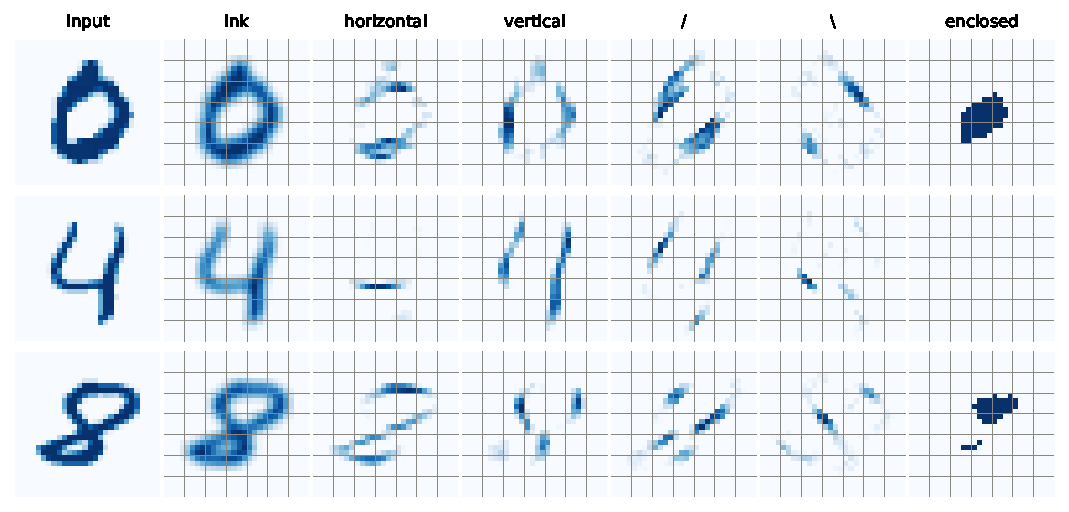
\includegraphics[width=\linewidth]{figures/holes_mnist_pipeline}
\caption{Three test digits through the network: the input, the five hand-drawn
convolution channels, and the output of the recurrent hole finder. The grid is the
$5\times5$ zone pooling. Note the 8 whose lower loop did not close: the single most
common error.}
\label{fig:holes-pipeline}
\end{figure}

\emph{Kernels.} Five $5\times5$ kernels: a $3\times3$ box blur for \emph{ink}, and
oriented-bar detectors for horizontal, vertical, ``/'' and ``\textbackslash'' strokes
($+1$ on the bar, $+1.5$ at the centre, $-0.25$ beside it, divided by 4, bias $-0.15$).
A stroke lights its own orientation and, because of the negative surround, not the
others.

\emph{Hole finder.} Holes---the enclosed background of a 0, 6, 8 or 9---are the strongest
single cue a person uses, and they are topological, which a feed-forward convolution
cannot compute. We compute them with a ReLU recurrence over the image. Let $b$ be the
background (ink below $0.3$). Seed $r_0$ with the border of $b$ and iterate
\[
r_{t+1} = \mathrm{relu}\big(\min(1,\textstyle\sum_{3\times3} r_t) + b - 1\big),
\]
so a background pixel becomes \emph{reached} as soon as it touches a reached pixel.
After 56 steps everything reachable from the border has been reached and $b-r$ is the
enclosed background. This is the same construction as the run-length counters of
Section~\ref{sec:text-quality}---a ReLU recurrence with identity self-connection---applied
over an image instead of a string.

\emph{Zone pooling.} All six maps (five conv channels and the hole map) are averaged over
a $5\times5$ grid of $4\times4$-pixel zones covering the central $20\times20$ box in which
MNIST digits sit: 150 zone features, plus seven globals (ink, hole area, hole area in
the top and bottom halves, width, height, left--right ink balance).

\emph{Sketches.} For each channel, each digit is drawn by hand on the $5\times5$ grid as
ASCII art (Figure~\ref{fig:holes-sketches}): \texttt{\#} strong, \texttt{+} some,
\texttt{.} little, \texttt{-} must be empty. The 60 sketches \emph{are} the weights of 60
units: a sketch $W$ gives the unit $W\cdot x-\tfrac12\|W\|^2$, which up to a constant is
minus the squared distance to the prototype, so the readout asks ``which hand-drawn
digit is this closest to'', channel by channel (channel weights: ink 1, strokes 2,
``\textbackslash'' 1, hole 4). The sketches were drawn after looking at what MNIST digits
look like at this resolution---slanted 1s, 4s with a stem to the right, 7s whose roof
sits on the second row---the way a person who has seen handwriting draws a digit, and
are deliberately coarse.

\begin{figure}[t]\centering
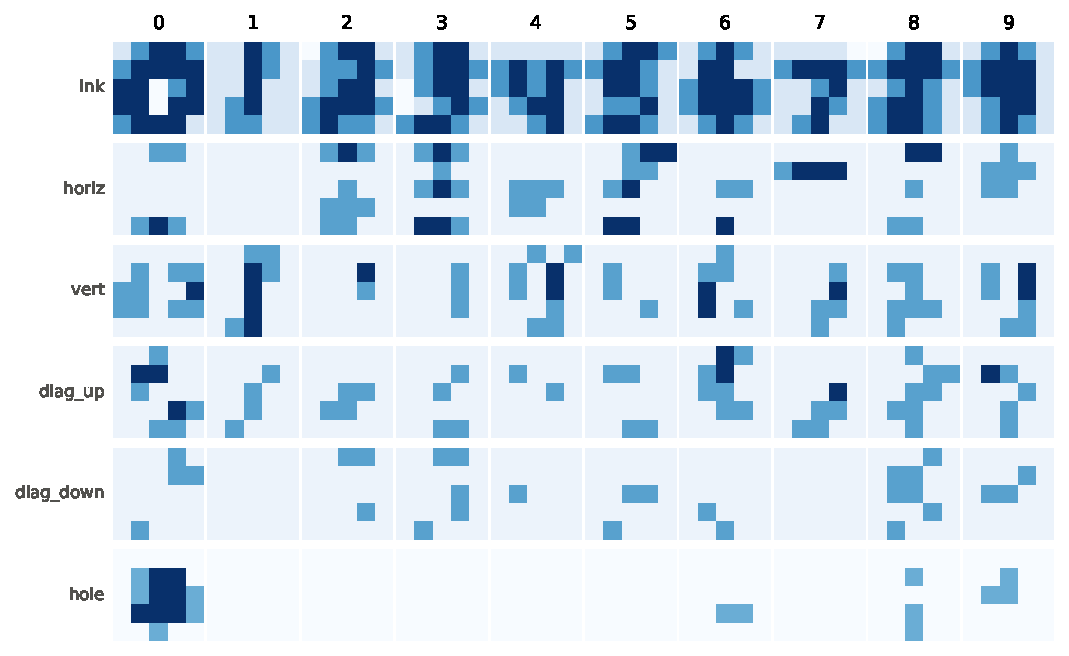
\includegraphics[width=\linewidth]{figures/holes_mnist_sketches}
\caption{The sixty hand-drawn sketches, one per digit and channel. These are the
prototype weights.}
\label{fig:holes-sketches}
\end{figure}

\emph{Evidence units.} Sketches alone reach about 80\,\%. The remaining confusions are
topological and shape facts that distance to a prototype does not capture, so 29 named
evidence units vote for and against digits, each a capped detector
$\min(\mathrm{relu}(w\cdot f+b),1)$ over a few zone features (the construction of
Section~\ref{sec:method-capped}): \texttt{hole:none} (votes for 1 3 4 5 7, against 0 8
9), \texttt{hole:big} (0), \texttt{hole:top\_only} (9), \texttt{hole:bottom\_only} (6),
\texttt{hole:top\_and\_bottom} (8), \texttt{narrow} (1), \texttt{four:open\_top} (two posts
and an empty top centre), \texttt{seven:roof}, \texttt{two:foot}, \texttt{three:bumps},
\texttt{five:corner}, \texttt{six:left\_sweep}, \texttt{nine:stem}, \texttt{zero:ring},
\texttt{eight:waist}, \texttt{bottom\_bar} (0 2 3 5 6 8 have one; 1 4 7 9 do not),
\texttt{roof\_row1} (a 7, never a 4), \texttt{top\_centre\_filled} (against 4),
\texttt{has\_horizontals} and \texttt{has\_backslashes} (against 1), and a few more.
In total $|\theta|=21{,}772$ and $\|\theta\|_0=2{,}411$.

\paragraph{How the numbers were set.} The kernels, the hole finder, the sketches and the
unit definitions were written from how digits look. Thresholds were placed by reading
class-conditional means of the zone features on the first 5{,}000 \emph{training} images
and putting the knee between a digit and its neighbours (``a 4's top-centre ink is 0.6, a
9's is 1.8, so threshold at 1.0''). Vote weights were then adjusted by hand over about a
dozen rounds of looking at the confusion matrix on those same 5{,}000 images and asking
which unit was to blame for each confusion. No gradient, optimiser or search over weights
was used. A held-out training slice (images 5{,}000--10{,}000) gives 82.8\,\%, so the hand
tuning did not overfit; the test set was scored once, at the end.

\paragraph{Results.} On the 10{,}000 MNIST test images the network is \textbf{83.3\,\%
accurate} (Figure~\ref{fig:holes-confusion}), at $0.9$\,ms per image in NumPy. The
majority class gives 11.4\,\%. A \emph{trained} nearest-class-mean classifier on the raw
784 pixels (ten prototypes fit on 20{,}000 training images) gives 81.6\,\%, so ten digits
drawn by hand on a $5\times5$ grid, plus the hole finder and a page of evidence, do
slightly better than ten prototypes fit to data at full resolution. A trained
convolutional network reaches over 99\,\%. Per-class accuracy ranges from 95\,\% (1) and
91\,\% (2, 3) down to 77\,\% (5, 9) and 65\,\% (8).

\begin{figure}[t]\centering
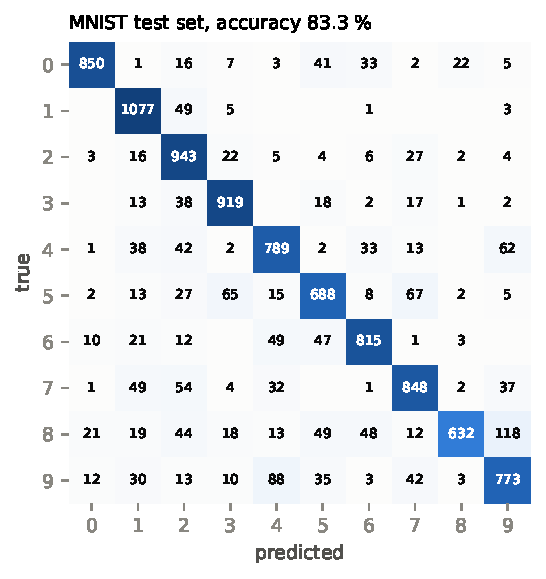
\includegraphics[width=0.5\linewidth]{figures/holes_mnist_confusion}
\caption{Confusion matrix on the 10{,}000 MNIST test images (rows normalised for colour).}
\label{fig:holes-confusion}
\end{figure}

\paragraph{Where it fails, by construction.} The errors are the ones a $5\times5$ sketch
would be expected to make, and the hole finder explains most of them: 8$\to$9 (118 cases)
when the lower loop did not close, 9$\to$4 (88) when the upper loop did not close,
4$\to$9 (62) when a 4 is written with a closed top; and the shape pairs 5$\to$7 (67) and
5$\leftrightarrow$3 (65), where a 5 with a short roof is a 3 with a corner. The unit
firing rates on the test set confirm the picture: \texttt{hole:none} fires on 99\,\% of 1s,
3s, 5s and 7s but also on 26\,\% of 9s and 37\,\% of 6s, which is where the accuracy
goes. A $5\times5$ sketch cannot say ``the loop must close'', and the hole finder cannot
close a loop the writer left open; a trained network learns the fine stroke-topology
statistics that fill that gap, and that is exactly the part of the task a designer
cannot write down.
